%%%%%%%%%%%%%%%%%%%%%%%%%%%%%%%%%%%%%%%%%%%%%%%%%%%%%%%%%%%%%%%%%%%
%                                                                 %
%                            CHAPTER                              %
%                                                                 %
%%%%%%%%%%%%%%%%%%%%%%%%%%%%%%%%%%%%%%%%%%%%%%%%%%%%%%%%%%%%%%%%%%%
\chapter{Evaluation}
\label{chapter:evaluation}

In this chapter we will take a look at the results of various experiments conducted during the process of making a secure CNN for face matching. First we describe our testing environment in order to make reproducible results. Then we move on by explaining our first experiment, where we sharpened an image with the help of convolutions of course we made a secure version of this algorithm, which keeps the input image and the convolution filters parameters private. Then we will test the complexity of each of the different layers of the network; convolution layer, subsampling layer and activation layer. Finally we discuss our obtained results and talk about the problems we came across.

\section{Testing Environment}
Following is a list of hardware and software used during testing the results can vary and depend on following items.

\paragraph{Hardware}
\begin{itemize}
  \item Machine: Lenovo ThinkPad T460s
  \item CPU: Intel Core i5-6300U (2.4 GHz)
  \item Memory: 8 GB DDR4
\end{itemize}

\paragraph{Software}
\begin{itemize}
  \item Windows 10 Pro (device) and Linux (servers)
  \item Python version 3.6
  \item Virtualization: Docker Desktop
  \item Database: MongoDB (NoSQL)
  \item Python packages: MPyC and Pytorch
\end{itemize}

To ensure that the secure face matching algorithm works as intended, all software listed below should be installed and the hardware should meet similar specifications as the hardware we used.

\section{Image Sharpening}
Image sharpening is a classic computer vision task. The task can be completed using convolutions. The process goes as follows: First we extract the horizontal lines or edges from an image by using a certain convolution mask (figure \ref{fig:sharp_mask}). We do the same thing for the vertical lines in the image. Adding these outputs gives us a detailed version of the input image, where only vertical and horizontal lines are left over. The detailed image than gets multiplied by a factor between 0 and 1. Finally the detailed image gets added to the input image, the result is a sharpened version of the original image.

\begin{figure}[H]
  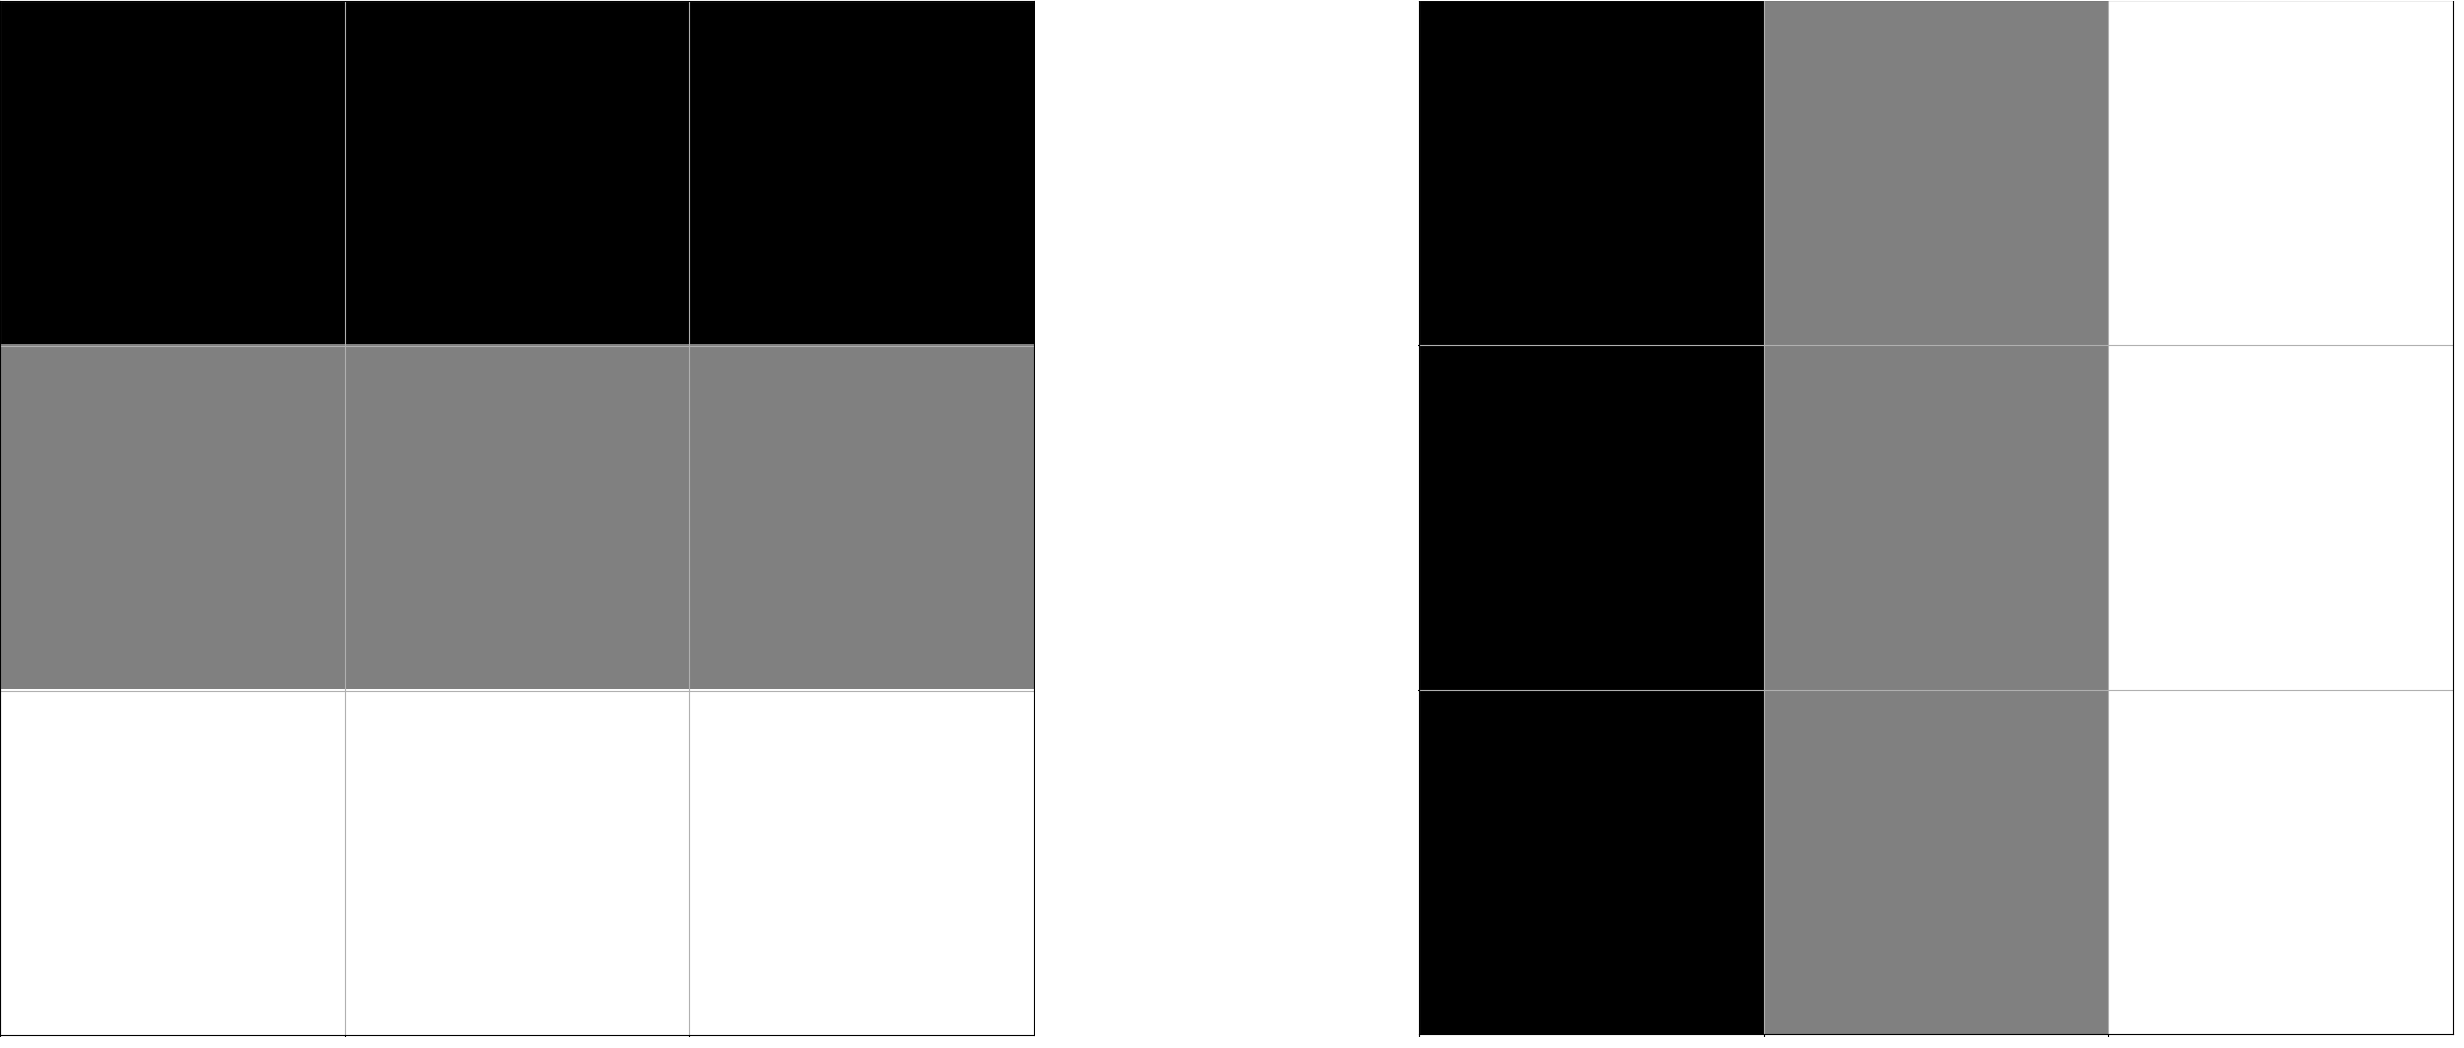
\includegraphics[scale=0.1]{fig/sharp_mask.png}
  \centering
  \caption{Convolution filters used for extracting sharp details out of images}
  \label{fig:sharp_mask}
\end{figure}

This demonstration nicely illustrates the possibilities for using secure convolutions and possibly other image processing tasks such as corner or edge detection. There are a total of two convolutions filters sized $3$x$3$. For an input image of size $100$x$100$ the total MPC running time which includes the two secure convolutions, the multiplication of the factor and the addition of the detailed images to the original images, equals to 60-80 seconds. For a bigger picture (figure \ref{fig:sharpened_image}), sized $640$x$360$, the computation takes much longer since the number of input pixels goes up drastically. The MPC computation time for those bigger pictures can take up to 5 minutes. An example of a securely sharpened image can be found below.

\begin{figure}[H]
  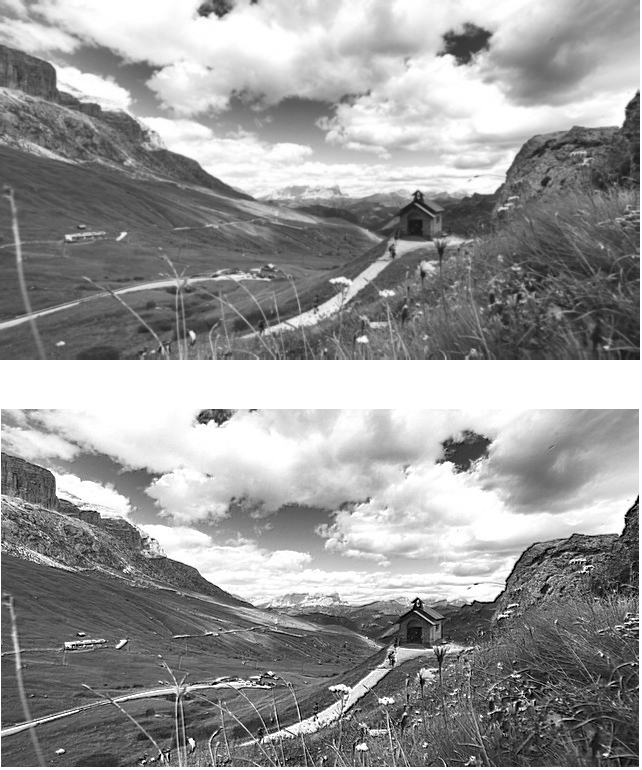
\includegraphics[scale=0.5]{fig/sharpened_image.png}
  \centering
  \caption{Convolution filters used for extracting sharp details out of images}
  \label{fig:sharpened_image}
\end{figure}

Notice that the contours and sharp lines in the original image are much more visible in the sharpened image. Let us revise what exactly happened from a security point of view. The client takes a picture with their device. Then they encrypt the picture, by using Shamir's secret sharing scheme. The secret shares of the encrypted image then gets sent to the appropriate three MPC servers. These servers now do the convolution to sharpen the image. Note that the parameters of the convolution filters are also encrypted, this means that the intellectual property of the algorithm stays protected. Of course this is not really useful for the image sharpening algorithm since it's publicly known what parameters are best chosen for the convolutions. But for algorithms that are not already known and would lose their value or income if they would be revealed, this feature would enable the parameters of those algorithms to stay private. After the server are done with the MPC protocol. The servers recombine their secret shares to get the output, the sharpened image.

\section{Complexity results}
In this section we show the complexity of the different secure operations (single convolution, max pooling and ReLU) and the different parts of the MPC protocol, secret sharing and share recombination for example. We do this by measuring how long it takes to perform the operation on a matrices with variable sizes. We then compare these results to their classic unencrypted equivalents.\\

We define our testing vector (the input image) as $I$ of size $s$x$s$, the kernel $K$ of size $3$x$3$ and the computation time $t$. Note that we only measure the computation time of one party. However that is fine, since the parties are running parallelized and they take around the same time to finish their computations.\\

The testing vector $I$ is randomly generated with values uniformly distributed over the range $[0,1]$.

\subsection{Convolution}
For this operation we have four different implementations as can be seen in figure \ref{fig:convolution_test}. The first one uses MPC to encrypt the input $I$. The second one uses MPC to encrypt both the image $I$ and the kernel $K$. The third convolution function is \codeword{torch.nn.Conv2d} from the Pytorch package. The last function is the cleartext equivalent of the MPC secure function but instead of using secret shares as input it only takes cleartext floating points and does not use the MPC framework.\\

The first two functions and the last function are defined in listing \ref{lst:convolution} of chapter \ref{Secure Functions}.

\begin{figure}[H]
  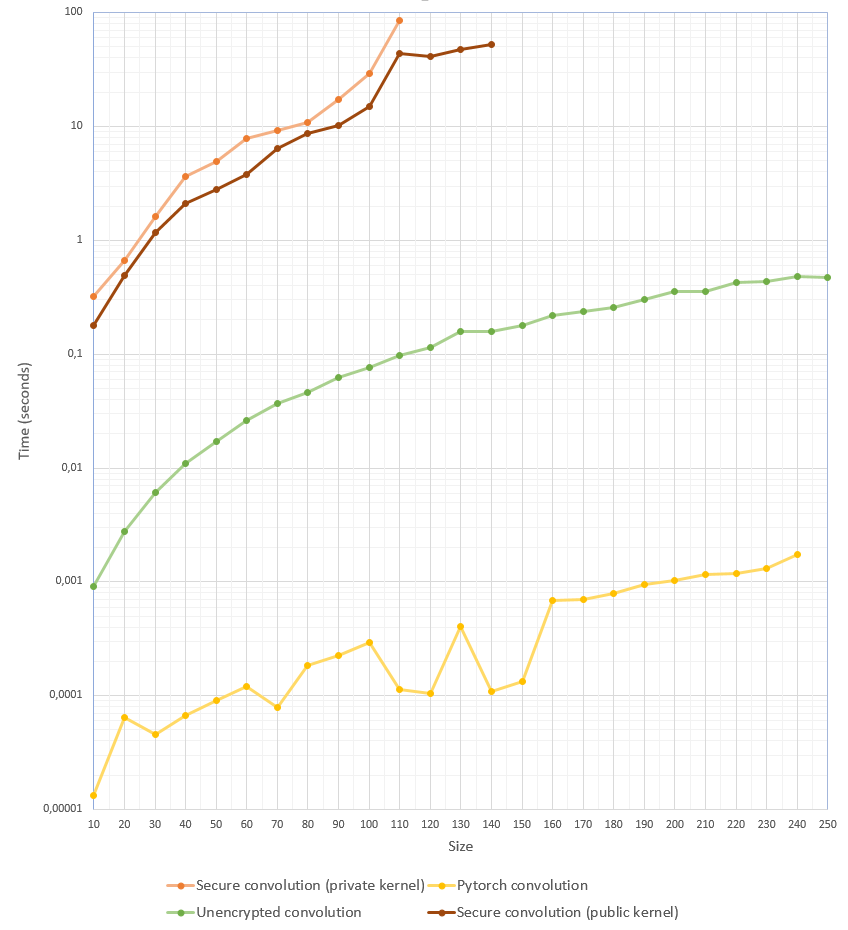
\includegraphics[scale=0.6]{fig/convolution_test.png}
  \centering
  \caption{Computation time for encrypted and unencrypted convolution functions}
  \label{fig:convolution_test}
\end{figure}

We observe that the Pytorch function is the fastest one of the four. The unencrypted convolution function is of a magnitude $10^2$ slower. The two other encrypted convolution take about the same time to complete. However, the convolution function where the kernel is also encrypted is a tad slower. This is logical, since communication between the MPC servers is needed for multiplication of two secrets (as seen in chapter \ref{Arithmetic operators}).

\subsection{Max Pooling}
In figure \ref{fig:maxpooling_test} three different max pooling functions are plotted over the size $s$ of the input $I$, while these functions are differently implemented the result is the same. The window size is $2$ and the stride is also $2$. The secure max pooling function uses MPC as means to encrypt the input $I$ and is defined in listing \ref{lst:maxpooling} of chapter \ref{Secure Functions}. The Pytorch max pooling function is \codeword{torch.nn.MaxPool2d} of the Pytorch package. The unencrypted max pooling function is the equivalent of the first encrypted function but instead of secret shares it uses cleartext floating points as input, and it does not utilize the MPC framework at all.

\begin{figure}[H]
  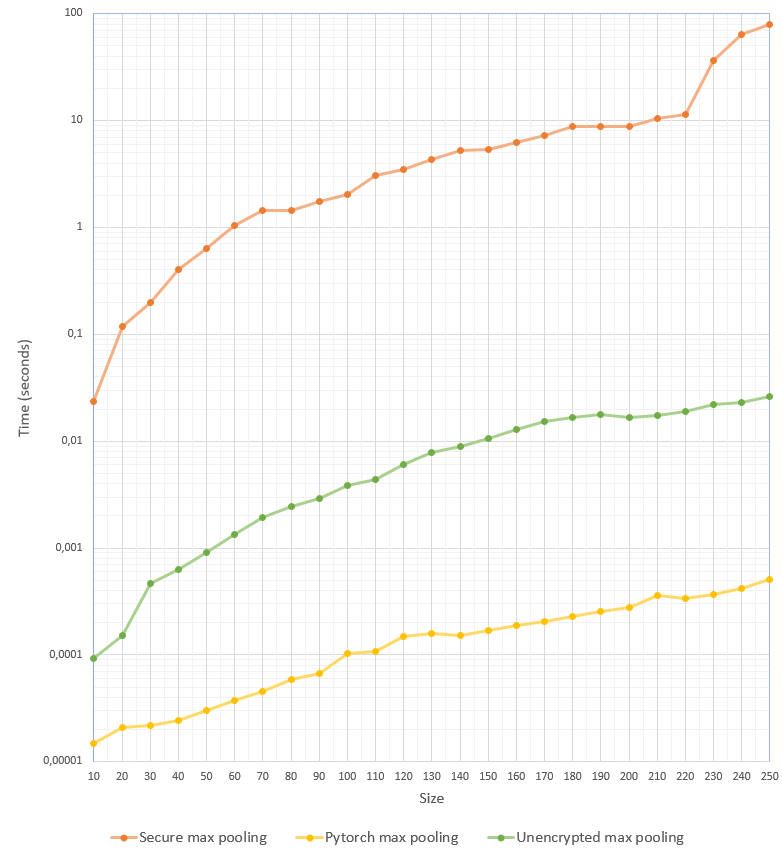
\includegraphics[scale=0.7]{fig/maxpooling_test.png}
  \centering
  \caption{Computation time for encrypted and unencrypted max pooling functions}
  \label{fig:maxpooling_test}
\end{figure}

We can clearly see that the Pytorch function is the most optimized function and runs the fastest. The unencrypted max pooling function is a factor of $10^1$ to $10^2$ slower. The MPC encrypted max pooling function is the slowest and reaches almost 100 seconds for max pooling over an image $I$ of size $s = 250$.

\subsection{ReLU}
In figure \ref{fig:relu_tests} three different functions are plotted for an image $I$ with sizes $s$ in range $s \in [10,250]$. The secure ReLU function is defined in listing \ref{lst:relu} of chapter \ref{Secure Functions} and uses MPC to encrypt the input $I$. The Pytorch ReLU function is \codeword{torch.nn.ReLU} from the Pytorch package. The results for this function shows very fast computation, this is because Pytorch is deeply integrated with C++ code. Finally, the unencrypted is the insecure equivalent of the first function but instead of using the MPC framework and giving secret shares as input, regular floating points are given as input.

\begin{figure}[H]
  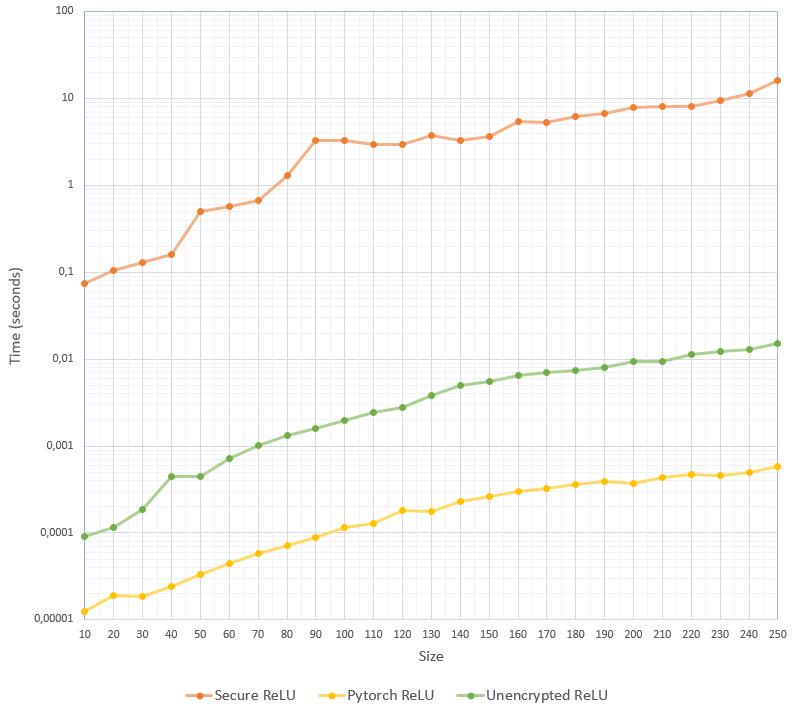
\includegraphics[scale=0.7]{fig/relu_tests.png}
  \centering
  \caption{Computation time for encrypted and unencrypted ReLU activation functions}
  \label{fig:relu_tests}
\end{figure}

The results are predictable, of course the Pytorch function is the fastest because of its utilization of C++ code. The unencrypted ReLU function is about ten times slower. The MPC secure function is about $10^4$ as slow as the Pytorch function and $10^3$ as slow as its unencrypted equivalent.

\subsection{Secret sharing and recombination}
Complexity analysis of Shamir's secret sharing scheme and secret recombination via Lagrange interpolation (chapter \ref{Secret sharing}) is less important than the other operations. Because they happen only once for every MPC instance, secret sharing happens at the beginning of the protocol while secret recombination takes place at the end. However they are essential parts of the MPC protocol. In our experiment (figure \ref{fig:secret_test} we let the computation of secret sharing happen on the device and secret recombination on the MPC servers. The time for those operations is measured for and image $I$ with size $s$ ranging from $10$ to $250$.

\begin{figure}[H]
  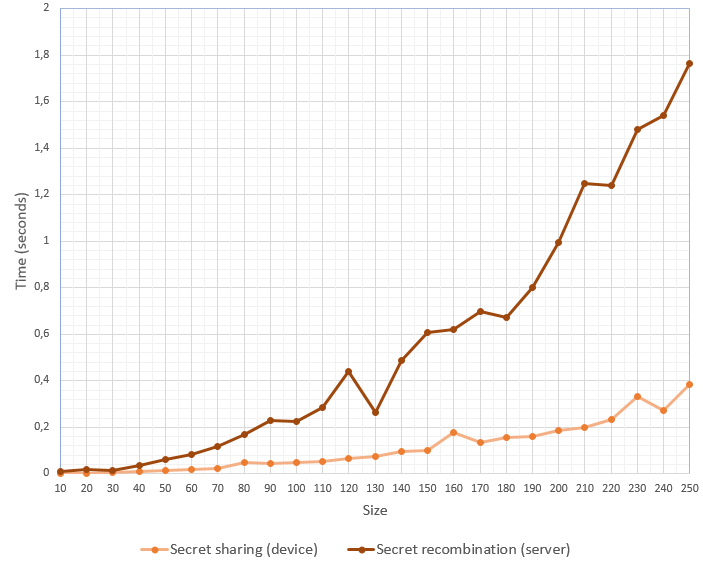
\includegraphics[scale=0.7]{fig/secret_test.png}
  \centering
  \caption{Computation time for secret sharing and recombination algorithms}
  \label{fig:secret_test}
\end{figure}

Notice that secret recombination takes more time, this is normal since communication between the parties is needed to publish the secret shares. Overall these operations are relatively fast (comparing to the other secure operations) and since they only occur once for every secure face matching task, their computation time is to be disregarded.

\section{Discussion \& Problems}
We had difficulties implementing the whole CNN in the MPC framework. To a point where it seemed impossible to continue. The docker containers running the MPC parties instances, crashed as soon as the computation began to be too complex. We couldn't figure out how to run multiple convolution layers after each other without crashing the system. We still have not figured out why a large input or a complex operation caused the docker containers to crash. Because of how difficult it is to backtrack the problem. We do not have enough experience regarding Docker. And since the goal of this thesis is not to master our debugging skills, we are sad to announce that we could not get the total secure face matching algorithm to work. However we have made significant progress by designing and testing the different secure methods needed for this face matching algorithm.\\

In theory our implementation is entirely feasible. But in practice more than just a couple of bright theoretical ideas are needed. For starters, a proper software stack that is indifferent to the size of the input or to the number of operations is much appreciated.\\

The crashes on the servers cause a connection timeout on the device. And happen in the following two cases (causes gathered from experience):

\begin{itemize}
  \item The number of input pixels is greater than 130x130 for a single convolution.
  \item The number of convolutions for an input of size 100x100 is greater than one.
\end{itemize}

These problems indicate that there is not enough memory available.\\

Another problem is the fact that the secure operations are very complex and take a lot of time to complete. An estimation of the total time it would take to complete one inference of the secure CNN in it's current form (without pruning) is calculated below (equation \ref{eq:comp_time}) taking into account the results from the computation time tests.\\

Secure face matching algorithm step per step:
\begin{itemize}
  \item 1 x secret sharing on $I$ with $s=100$
  \item 4 x single convolution on $I$ with $s=100$
  \item 4 x max pooling on $I$ with $s=98$
  \item 4 x ReLU on $I$ with $s=49$
  \item 32 x single convolution on $I$ with $s=49$
  \item 8 x max pooling on $I$ with $s=47$
  \item 8 x ReLU on $I$ with $s=23$
  \item 64 x single convolution on $I$ with $s=23$
  \item 8 x max pooling on $I$ with $s=21$
  \item 8 x ReLU on $I$ with $s=10$
  \item 8 x secret recombination on $I$ with $s=10$
\end{itemize}

\begin{equation} \label{eq:comp_time}
  \begin{aligned}
      t_{total} = & 1\times0.0476166 + 4\times14.8732678 + 4\times2.0341087 + 4\times0.4950582\\
                & + 32\times2.792582 + 8\times0.6305378 + 8\times0.1049295 + 64\times0.4898818\\
                & + 8\times0.1172477 + 8\times0.073816 + 8\times 0.0109198\\
      t_{total} = & 197.872021
  \end{aligned}
\end{equation}

The total computation time for one inference through the secure CNN is approximately 198 seconds. This however, seems pretty optimistic. We are sure some elements like parties waiting on each other are not taken into account. But since we do not have a practical working implementation of the secure face matching algorithm we can not say for certain how long it would take to complete one task. From what we know, we can say that one inference takes at least than 3 minutes and the total timings in practice could range from 5 to 15 minutes\footnote{Based from the information we gathered while working on the algorithm}.
